\documentclass[12pt,a4paper]{article}
\usepackage[brazil]{babel}
\usepackage[utf8]{inputenc}
\usepackage[T1]{fontenc}
\usepackage{graphicx}


\usepackage{color}
\definecolor{codegreen}{rgb}{0,0.6,0}
\definecolor{codegray}{rgb}{0.5,0.5,0.5}
\definecolor{codepurple}{rgb}{0.58,0,0.82}
\definecolor{backcolour}{rgb}{0.95,0.95,0.92}

\usepackage{listings}
\lstset{ 
    language=Haskell,
    backgroundcolor=\color{backcolour},   
    commentstyle=\color{codegreen},
    keywordstyle=\color{magenta},
    numberstyle=\tiny\color{codegray},
    stringstyle=\color{codepurple},
    basicstyle=\footnotesize,
    breakatwhitespace=false,         
    breaklines=true,                 
    captionpos=b,                    
    keepspaces=true,                                                  
    showspaces=false,                
    showstringspaces=false,
    showtabs=false,                  
    tabsize=2
}

\title{Ordenação em Haskell}
\author{Bruno Tatsuya Masunaga Santos\\
        Paradigmas de Programação 2018.2}
\date{\today}

\begin{document}
\maketitle

\section{Introdução}
Com o objetivo de estudar a ordenação de listas em Haskell, analisando seu desempenho em diversos casos, foram implementados alguns dos principais algoritmos conhecidos em Computação. Utilizou-se, para tanto, funcionalidades da linguagem de programação funcional Haskell e de conhecimentos adquiridos durante as aulas da disciplina Paradigmas de Programação, ofertada pela UFABC e ministrada pelo Prof. Fabrício Olivetti. 

\section{Metodologia}
Para o desenvolvimento deste projeto, foi realizada primeiramente a implementação de nove algoritmos de ordenação, a saber: Bubble Sort, Insertion Sort, Selection Sort, Merge Sort, Quick Sort, Counting Sort, Heap Sort, Bucket Sort e Radix Sort. A implementação de cada um desses algoritmos possui peculiaridades que serão discutidas mais adiante. Concluídas as implementações, utilizou-se o artifício QuickCheck para garantir o funcionamento correto das funções declaradas e, portanto, validando os algoritmos desejados.

Todos os algoritmos foram submetidos à execução da ordenação de 20 listas diferentes, e o tempo de avaliação para cada caso foi mensurado. Desta forma, elaborou-se análises estatísticas a partir do estudo da variação do tempo de avaliação dos algoritmos em função do tamanho da lista utilizada, tornando possível realizar algumas comparações entre as implementações criadas.

\section{Implementação dos Algoritmos}
As implementações de todos os algoritmos pode ser vista em \textbf{src/Sorting.hs}. Em todos os casos, optou-se por realizar uma tradução dos passos de cada algoritmo para a linguagem Haskell e, de fato, essa foi a tarefa mais difícil. Devido às características intrínsecas do Haskell, como imutabilidade e avaliação preguiçosa, muitos dos algoritmos foram implementados de modo que perderam sua eficiência original (muitas vezes dada pela implementação imperativa), como será visto mais para frente. É importante ressaltar que todos os algoritmos foram implementados para efetuar a ordenação em ordem crescente de elementos.

Para utilizar qualquer um destes algoritmos, basta carregar o arquivo \textbf{src/Sorting.hs} no GHCI. A função correspondente respeita o padrão CamelCase. Veja abaixo um exemplo prático:

\begin{figure}[h]
	\centering
	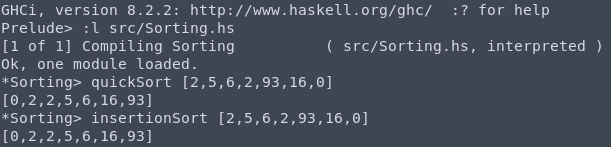
\includegraphics[scale=0.5]{images/sortingExample.png}
	\caption{Exemplo de utilização dos algoritmos implementados}
\end{figure}

\subsection{Bubble Sort}
O Bubble Sort é um algoritmo de ordenação simples. Percorre o vetor muitas vezes, de modo a realizar trocas até que ele esteja ordenado, carregando os elementos para sua posição correta. De acordo com sua implementação imperativa, sua complexidade no pior caso é O($n^2$). 

A implementação em Haskell apresentada neste projeto foi realizada pelo autor. As funções envolvidas são:
\begin{itemize}
\item \textbf{ordenado}: Verifica se uma lista está ordenada.
\item \textbf{chamadaBubble}: Realiza a troca entre elementos se o primeiro da lista recebida é maior do que o segundo. Além disso, faz chamada da função \textbf{bubbleSort}.
\item \textbf{bubbleSort}: Recebe uma lista, verifica se ela está ordenada, chamando \textbf{ordenado}. Se sim, então retorna a lista que recebeu. Se não, chama a função \textbf{chamadaBubble}. 
\end{itemize}
Neste caso, foi utilizado o conceito de Recursão Mútua entre \textbf{chamadaBubble} e \textbf{bubbleSort}. 

A assinatura da função principal é dada por:

\begin{lstlisting}
bubbleSort :: (Ord a) => [a] -> [a]
\end{lstlisting}

Portanto, este algoritmo é capaz de ordenar qualquer tipo de lista que contenha elementos da classe Ord. Veja abaixo alguns exemplos:

\begin{figure}[h]
	\centering
	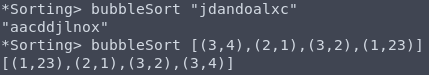
\includegraphics[scale=0.6]{images/bubbleExample.png}
	\caption{Exemplos de utilização do Bubble Sort}
\end{figure}

\subsection{Insertion Sort}
O Insertion Sort também é um algoritmo simples. Ele funciona basicamente inserindo cada elemento em sua posição correta. De acordo com sua implementação imperativa, sua complexidade no pior caso é O($n^2$). 

A implementação em Haskell apresentada neste projeto foi adaptada das aulas da disciplina. As funções envolvidas são:

\begin{itemize}
\item \textbf{inserir}: Recebe um elemento e uma lista. Insere este elemento recursivamente na posição correta na lista.
\item \textbf{insertionSort}: Recebe uma lista e chama \textbf{inserir} a cada chamada recursiva.
\end{itemize}

A assinatura da função principal é dada por:

\begin{lstlisting}
insertionSort :: (Ord a) => [a] -> [a]
\end{lstlisting}

Portanto, assim como o Bubble Sort, este algoritmo consegue ordenar qualquer tipo de lista que contenha elementos da classe Ord.


\subsection{Selection Sort}
O Selection Sort é um algoritmo simples. Ele percorre o vetor uma vez, obtendo o menor elemento na lista cada vez que avança, alocando-o na posição correta. De acordo com sua implementação imperativa, sua complexidade no pior caso é O($n^2$). 

A implementação em Haskell apresentada neste projeto foi realizada pelo autor. As funções envolvidas são:

\begin{itemize}
\item \textbf{remover}: Recebe um elemento e uma lista. Remove este elemento desta lista.
\item \textbf{selectionSort}: Remove o mínimo elemento da lista e aloca-o na primeira posição. Faz a chamada recursiva para o restante da lista.
\end{itemize}

A assinatura da função principal é dada por:

\begin{lstlisting}
selectionSort :: (Ord a) => [a] -> [a]
\end{lstlisting}

Logo, consegue ordenar qualquer tipo de lista que contenha elementos da classe Ord.


\subsection{Merge Sort}
O Merge Sort é um algoritmo ótimo. Ele divide recursivamente o vetor em sua metade. A cada volta da chamada recursiva, faz a intercalação entre as duas metades, ordenando a lista parte a parte. De acordo com sua implementação imperativa, sua complexidade no pior caso é O($n\log n$). 

A implementação em Haskell apresentada neste projeto foi adaptada das aulas da disciplina. As funções envolvidas são:

\begin{itemize}
\item \textbf{intercalar}: Recebe duas listas ordenadas e retorna uma lista ordenada que contenha as duas listas de entrada.
\item \textbf{dividir}: Recebe uma lista e divide-a em duas metades.
\item \textbf{mergeSort}: Recebe uma lista, divide-a recursivamente em duas metades e intercala recursivamente as duas metades para cada chamada.
\end{itemize}

A assinatura da função principal é dada por:

\begin{lstlisting}
mergeSort :: Ord a => [a] -> [a]
\end{lstlisting}

Como todos os anteriormente citados, consegue ordenar qualquer tipo de lista que contenha elementos da classe Ord.

\subsection{Quick Sort}
O Quick Sort é considerado um dos melhores algoritmos de ordenação. Ele se baseia no particionamento recursivo inteligente, organizando todos os elementos maiores do que um dado elemento de um lado e todos os elementos menores do outro. De acordo com sua implementação imperativa, sua complexidade no pior caso é O($n^2$). No entanto, isso só ocorre quando o vetor está reversamente ordenado. Na grande maioria das vezes, sua complexidade é dada por O($n\log n$). 

A implementação em Haskell apresentada neste projeto foi adaptada das aulas da disciplina. As funções envolvidas são:

\begin{itemize}
\item \textbf{dividirPivot}: Realiza o particionamento inteligente de uma lista utilizando o primeiro elemento.
\item \textbf{quickSort}: Recursivamente, chama o particionamento inteligente e concatena as listas parciais já ordenadas.
\end{itemize}

A assinatura da função principal é dada por:

\begin{lstlisting}
quickSort :: (Ord a) => [a] -> [a]
\end{lstlisting}

Mais uma vez, temos um algoritmo que consegue ordenar qualquer tipo de lista que contenha elementos da classe Ord.

\subsection{Counting Sort}
O Counting Sort é um algoritmo de ordenação considerado bom para situações específicas. O algoritmo faz uso de memória auxiliar de acordo com o intervalo de dados presentes no vetor. Desta forma, ele literalmente conta quantas vezes cada elemento aparece no vetor, criando, por final, um vetor ordenado. De acordo com sua implementação imperativa, sua complexidade no pior caso é O($n+k$), de modo que k é o maior valor do vetor.

A implementação em Haskell apresentada neste projeto não é a versão original do Counting Sort. Devido às características do Haskell, optou-se por realizar a implementação de uma variação do Counting Sort, cuja diferença é que no final, o algoritmo percorre o vetor auxiliar para criar diretamente um novo vetor ordenado. Essa implementação foi realizada pelo autor. As funções envolvidas são:

\begin{itemize}
\item \textbf{tamanhoAuxiliar}: Determina o tamanho do vetor auxiliar com base no maior e menor valor de uma lista recebida.
\item \textbf{contarOcorrencias}: Dado um elemento e uma lista, conta quantas vezes este elemento aparece nesta lista.
\item \textbf{construirAuxiliar}: Constrói o vetor auxiliar com as devidas ocorrências de cada elemento, utilizando as duas funções anteriores.
\item \textbf{adicionar}: Recebe um valor e um número i. Cria uma lista com i elementos iguais a esse valor. 
\item \textbf{countingSort}: A partir de uma lista recebida, concatena os elementos de uma lista de listas, criada pela utilização da função \textbf{adicionar} para cada elemento do vetor auxiliar construído por \textbf{construirAuxiliar}.
\end{itemize}

A assinatura da função principal é dada por:

\begin{lstlisting}
countingSort :: [Int] -> [Int]
\end{lstlisting}

Este algoritmo, dada sua implementação, apenas pode ser utilizado para ordenar inteiros, uma vez que o tamanho do vetor auxiliar depende dos valores máximo e mínimo da lista a ordenar.

\subsection{Heap Sort}
O Heap Sort é algoritmo de ordenação ótimo. Utiliza-se de uma estrutura de dados chamada Heap, que permite organização dos dados de um vetor de modo que ao percorrê-lo, visite apenas metade de seus elementos, dependendo do contexto. De acordo com sua implementação imperativa, sua complexidade no pior caso é O($n\log n$).

A implementação em Haskell teve o maior nível de dificuldade dentre os algoritmos escolhidos. Neste caso, utilizou-se a versão Max-Heap Sort do algoritmo, que utiliza um Heap Máximo. O código foi adaptado de variadas fontes da Web, que incluem GitHub e RosettaCode. As funções envolvidas são:

\begin{itemize}
\item \textbf{trocar}: Recebe o índice de dois elementos e uma lista. Troca estes elementos de posição caso o de menor índice seja maior.
\item \textbf{encontrarMaximo}: Dado o índice de um nó pai, compara seu valor com o de seus filhos e retorna o índice de qual dos três é o maior.
\item \textbf{maxHeapify}: Recursivamente, faz com que o maior valor entre um pai e seus filhos seja o pai.
\item \textbf{construirHeap}: Constrói o Heap de Máximo imaginário com base na lista de entrada.
\item \textbf{chamadaHeap}: Coordena as chamadas recursivas de trocar os elementos e ordená-los do maior para o menor, excluindo-os de uma nova análise.
\item \textbf{heapSort}: Faz a primeira chamada de \textbf{chamadaHeap}, passando como parâmetro o Heap construído por \textbf{construirHeap}.
\end{itemize}

A assinatura da função principal é dada por:

\begin{lstlisting}
heapSort :: (Ord a) => [a] -> [a]
\end{lstlisting}

E logo, é um algoritmo capaz de ordenar qualquer lista de elementos do tipo Ord.


\subsection{Bucket Sort}
O Bucket Sort é um algoritmo que não realiza trocas ou comparações entre os elementos de um vetor. Ele divide os elementos em "baldes" (buckets), que representam um intervalo determinado de valores, ordena os elementos de cada balde e constrói o vetor ordenado apenas recuperando os valores. De acordo com sua implementação imperativa, sua complexidade no pior caso é O($n^2$), mas seu caso médio é dado por O($n \log n$), que é mais recorrente.

Existem muitas variações deste algoritmo. Nesta implementação para o Haskell, optou-se por utilizar 10 buckets e o Insertion Sort como subrotina para ordenar os buckets. Esse modelo é uma adaptação da variação Generic Bucket Sort, que utiliza n buckets, onde n é um número calculado que depende do valor máximo do vetor. Essa implementação foi realizada pelo autor. As funções envolvidas são:

\begin{itemize}
\item \textbf{divisor}: Calcula o divisor adequado para que cada elemento caia dentro de um dos 10 buckets.
\item \textbf{encontrarBucket}: Dado um elemento e a lista a qual ele pertence, encontra o bucket para o qual ele será alocado.
\item \textbf{criarBucket}: Cria um dos buckets com os elementos que ele possui de acordo com uma lista de entrada.
\item \textbf{criarBuckets}: Devolve uma lista de listas, que representa o conjunto dos 10 buckets com seus devidos elementos.
\item \textbf{ordenarBuckets}: Aplica o Insertion Sort em cada bucket, para ordená-los.
\item \textbf{bucketSort}: Concatena os elementos da lista de buckets ordenados, criados pela associação de todas as funções anteriores.
\end{itemize}

A assinatura da função principal é dada por:

\begin{lstlisting}
bucketSort :: [Int] -> [Int]
\end{lstlisting}

Embora a assinatura permita entrar com uma lista de quaisquer inteiros, este algoritmo só pode ser utilizado para ordenar inteiros não-negativos. Não foi possível encontrar uma maneira de restringir esta assinatura. Essa exceção se dá pelo fato de que um número negativo não cairá em nenhum dos buckets de acordo com esta implementação.

\begin{figure}[h]
	\centering
	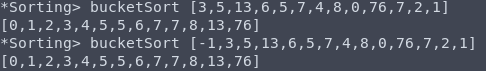
\includegraphics[scale=0.6]{images/bucketLimitation.png}
	\caption{Demonstração da Limitação do Bucket Sort}
\end{figure}


\subsection{Radix Sort}
O Radix Sort é um algoritmo que aplica análise de dígitos. Ele ordena dígito a dígito todos os elementos de um vetor. De acordo com sua implementação imperativa, sua complexidade no pior caso é O($nk$), onde k é o número de dígitos do maior número.

Existem dois tipos principais de Radix Sort: o MSD, que começa a ordenação a partir do dígito mais significativo, e o LSD, que começa a ordenação a partir do dígito menos significativo. Optou-se por utilizar a versão LSD. No algoritmo original, utiliza-se o Counting Sort como subrotina para ordenar os dígitos. No entanto, não foi possível utilizar este algoritmo, uma vez que, da maneira a qual foi implementado, o Radix Sort necessitava de um algoritmo que ordenasse tuplas. Como visto anteriormente, o Counting Sort implementado neste projeto apenas ordena inteiros. Desta forma, utilizou-se o Selection Sort. A implementação foi realizada pelo autor. As funções envolvidas são:

\begin{itemize}
\item \textbf{maiorElemento}: Retorna o maior elemento de uma lista. 
\item \textbf{numDigitos}: Retorna o número de dígitos que o maior elemento da lista possui.
\item \textbf{obterDigito}: Dado um número e a numeração de um dígito específico (da direita para a esquerda começando em 1), retorna o dígito deste número.
\item \textbf{obterDigitos}: Dada uma lista e a numeração de um dígito específico, retorna uma lista de tuplas, compostas pelo dígito obtido deste número e seu índice na lista original.
\item \textbf{ordenarDigitos}: A partir da lista de tuplas obtida por \textbf{obterDigitos}, aplica o Selection Sort e devolve uma lista de índices, que indicam qual posição cada elemento da lista original deve ficar.
\item \textbf{recuperarNumeros}: Dada a lista de índices ordenados gerada por \textbf{ordenarDigitos}, constrói a lista ordenada com os elementos originais.
\item \textbf{chamadaRadix}: Dada uma lista e uma numeração de dígito específico, ordena a lista em relação a este dígito.
\item \textbf{radix}: Controla as chamadas recursivas de \textbf{chamadaRadix}, garantindo que os números sejam ordenados do dígito menos significativo para o mais significativo.
\item \textbf{radixSort}: Faz a primeira chamada de \textbf{chamadaRadix}.
\end{itemize}

A assinatura da função principal é dada por:

\begin{lstlisting}
radixSort :: [Int] -> [Int]
\end{lstlisting}

Novamente, embora a assinatura permita entrar com uma lista de quaisquer inteiros, este algoritmo só pode ser utilizado para ordenar inteiros não-negativos. Essa exceção se dá pelo fato de que o algoritmo não reconhece o sinal negativo, considerando-o um dígito maior do que qualquer número.

\begin{figure}[h]
	\centering
	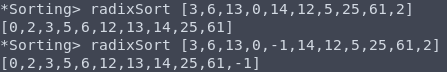
\includegraphics[scale=0.6]{images/radixLimitation.png}
	\caption{Demonstração da Limitação do Radix Sort}
\end{figure}

\section{Validação com o QuickCheck}
Para verificar a funcionalidade correta dos algoritmos, foi utilizada a biblioteca QuickCheck. Como visto em aula, os algoritmos de ordenação possuem certas propriedades, as quais podem ser implementadas e testadas pela biblioteca citada. São elas:
\begin{itemize}
\item \textbf{Idempotência}: O resultado da aplicação da função de ordenação uma única vez é igual ao resultado de várias aplicações sucessivas sobre o mesmo vetor.
\item \textbf{Tamanho igual}: O tamanho do vetor desordenado deve ser igual ao tamanho do vetor ordenado.
\item \textbf{O primeiro é o menor}: O valor mínimo do vetor desordenado é igual ao primeiro valor do vetor ordenado.
\end{itemize}

Essas propriedades foram implementadas em Haskell como funções, de modo que, para cada algoritmo, suas assinaturas acompanham a assinatura do método analisado. Veja a forma geral para um algoritmo que ordena qualquer vetor de elementos Ord:

\begin{lstlisting}
p1 :: (Ord a) => [a] -> Bool
p1 xs = (algoritmo $ algoritmo xs) == algoritmo xs

p2 :: (Ord a) => [a] -> Bool
p2 xs = (length $ algoritmo xs) == length xs

p3 :: (Ord a) => [a] -> Property
p3 xs = not (null xs)
        ==> (head $ algoritmo xs) == minimum xs
\end{lstlisting}

Onde \textbf{p1} se refere à propriedade da idempotência, \textbf{p2} se refere à propriedade do tamanho e \textbf{p3} se refere à propriedade do mínimo. Veja que \textbf{algoritmo} se refere a todos os algoritmos de ordenação que ordenam vetores de elementos Ord.


Para o Counting Sort, Bucket Sort e Radix Sort, a assinatura dessas funções foram dadas da seguinte maneira: 
\begin{lstlisting}
p1 :: [Int] -> Bool
p2 :: [Int] -> Bool
p3 :: [Int] -> Property
\end{lstlisting}

Todos os algortimos foram validados pelas três propriedades com sucesso pelo QuickCheck, com exceção do Bucket Sort e do Radix Sort. Como citado anteriormente, a assinatura dada para essas duas funções não é a ideal, uma vez que esses algoritmos, pela maneira que foram implementados, falham para números negativos. No entanto, não se soube implementar um método para limitar corretamente os parâmetros de entrada nestes algoritmos.

Para fazer a verificação das propriedades dos algoritmos, basta carregar o arquivo \textbf{src/Validate.hs} no GHCI utilizando o \textbf{stack} e chamar a função \textbf{quickCheck} seguida da propriedade desejada. Neste arquivo, as propriedades estão declaradas para cada algoritmo, e estão identificadas pela letra inicial de seu nome, com exceção de Bucket Sort, que carrega as letras "bk". Veja abaixo um exemplo com a seguinte sequência de comandos:

\begin{lstlisting}
$ stack ghci src/Validate.hs
$ quickCheck p1c
$ quickCheck p2c
$ quickCheck p3c
$ quickCheck p1bk
\end{lstlisting}

Esta sequência avalia as três propriedades para Counting Sort e a primeira propriedade para o Bucket Sort. O resultado obtido é:

\begin{figure}[h]
	\centering
	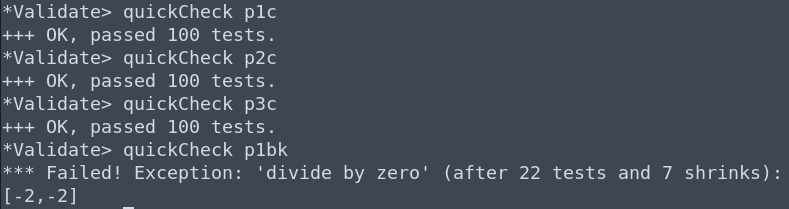
\includegraphics[scale=0.5]{images/quickCheck.png}
	\caption{Utilização do QuickCheck para verificar o Counting Sort e falha para Bucket Sort}
\end{figure}

\section{Comparação entre os algoritmos}
Para realizar uma comparação de eficiência temporal dos algoritmos implementados, foram realizados testes de performance para cada um utilizando listas de números inteiros não-negativos de tamanho e organização variados. Basicamente, foram gerados vetores de 4 comprimentos diferentes: 100, 1000, 10000 e 20000. Para cada comprimento, foram gerados 5 vetores que diferem em sua organização: ordenado (Sorted), reversamente ordenado (Reverse), todos elementos iguais (Equal), aleatório com pequeno intervalo (Little Rand) e aleatório com grande intervalo (Big Rand). Os vetores gerados podem ser verificados em \textbf{input/inputs.txt}.

Também foi incluída na análise de testes a função de ordenação padrão do Haskell, o \textbf{sort}, presente em \textbf{Data.List}, com o objetivo de verificar se esta função é a mais eficiente.

Foram utilizadas funções especiais para esta parte do projeto, ambas presentes em \textbf{Data.Time}:

\begin{itemize}
\item \textbf{getCurrentTime}: Captura o horário UTC atual.
\item \textbf{diffUTCTime}: Calcula a diferença, em segundos, entre dois horários UTC capturados pela função anterior.
\end{itemize}

Para cada algoritmo, foi utilizado o comando \textbf{evaluate} do Haskell, para que houvesse avaliação da função mas não houvesse impressão da lista ordenada. O código para avaliação de todos os algoritmos seguiu o seguinte modelo:

\begin{lstlisting}
start <- getCurrentTime
evaluate $ algoritmo array
end <- getCurrentTime
let dif = diffUTCTime end start
print ("Algoritmo: " ++ show dif)
\end{lstlisting}

Onde \textbf{start} é o horário UTC capturado antes da avaliação da execução do algoritmo, \textbf{end} é o horário UTC capturado depois da conclusão da avaliação do algoritmo, \textbf{dif} é o tempo transcorrido entre o começo e o fim do algoritmo, \textbf{algoritmo} é o método de ordenação avaliado e \textbf{array} é a lista de teste utilizada.

Essa parcela de código pode ser verificada em \textbf{src/Main.hs}.

\subsection{Avaliando o tempo de ordenação de uma lista arbitrária para todos os algoritmos}
Qualquer lista pode ser avaliada por todos os algoritmos de uma só vez utilizando o método explicado anteriormente, desde que seja uma lista de inteiros não-negativos (devido à limitação do Bucket Sort e do Radix Sort). Para tanto, basta atribuir a lista desejada ao nome \textbf{array} no arquivo \textbf{src/Main.hs} e executar o projeto. 

Como exemplo, vamos efetuar a avaliação para a seguinte lista:
\begin{lstlisting}
[2,4,13,35,6,54,213,16,7,8,0,0,1]
\end{lstlisting}
Primeiramente, vamos declará-la em \textbf{src/Main.hs}, atribuindo-a para \textbf{array}:

\begin{figure}[h]
	\centering
	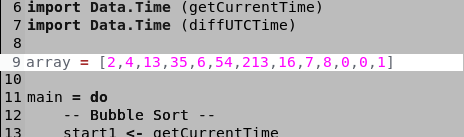
\includegraphics[scale=0.5]{images/mainVectExample.png}
	\caption{Atribuindo a lista desejada para array}
\end{figure}
Após salvar o arquivo, utilizar os seguintes comandos:

\begin{lstlisting}
$ stack setup
$ stack build
$ stack exec sorths
\end{lstlisting}

O resultado será:
\pagebreak
\begin{figure}[t]
	\centering
	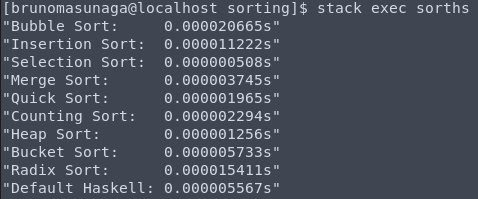
\includegraphics[scale=0.6]{images/execExample.png}
	\caption{Resultado da avaliação para a lista desejada}
\end{figure}

\subsection{Resultados da análise dos 20 vetores gerados}
Foram elaborados gráficos para comparar o tempo de execução de cada algoritmo para cada família de vetores de mesmo tamanho. No entanto, os dados referentes ao Bubble Sort não foram representados por destoarem muito, portanto, serão apresentados separadamente. Para os 4 tamanhos de vetores, foram elaborados 2 gráficos: o primeiro demonstrando uma visão geral do desempenho de todos os algoritmos e o segundo com enfoque nos algoritmos que levaram menos tempo. Todos os testes foram realizados num Intel Core i7-4500U de 1.80GHz com 8GB RAM em situações de uso exclusivo do computador e podem ser verificados no diretório \textbf{output/}.

Os resultados obtidos para os vetores de tamanho 100 podem ser vistos nas imagens abaixo:
\begin{figure}[h]
	\centering
	\fbox{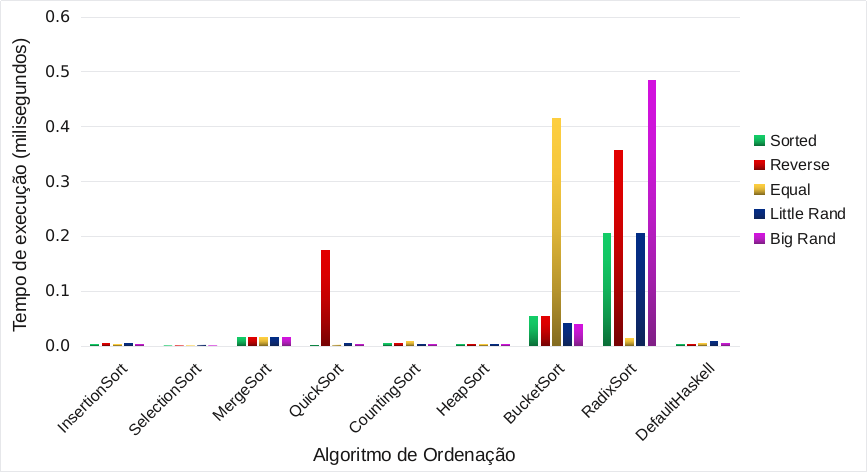
\includegraphics[scale=0.4]{images/result100-b.png}}
	\caption{Desempenho dos algoritmos para vetores de tamanho 100}
\end{figure}

\pagebreak

\begin{figure}[h]
	\centering
	\fbox{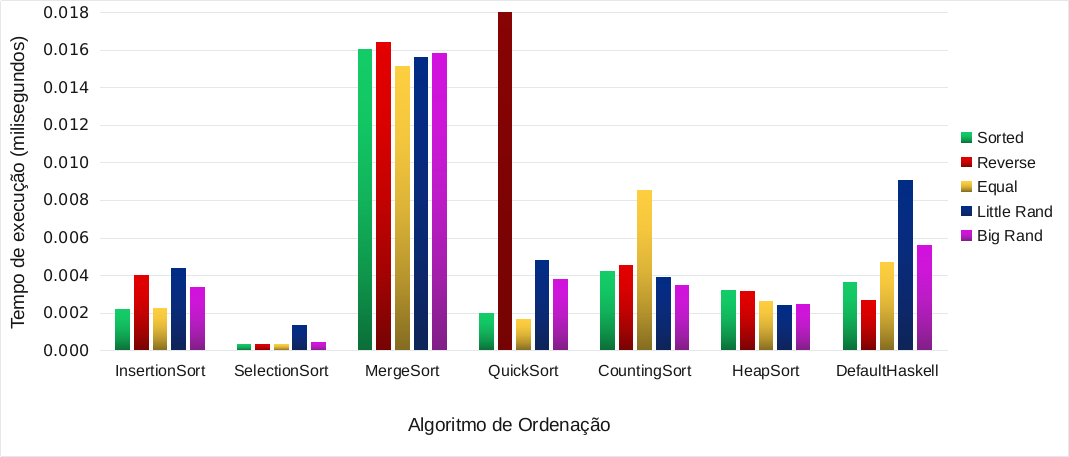
\includegraphics[scale=0.35]{images/result100-bbkr.png}}
	\caption{Desempenho dos algoritmos mais eficientes para vetores de tamanho 100}
\end{figure}

Neste caso, a média de tempo de execução do Bubble Sort foi de aproximadamente 1.39 ms, cerca de 5 vezes mais lento que o Radix Sort e cerca de 2400 vezes mais lento que o Selection Sort, que foi o algoritmo mais rápido neste teste.

Agora, vejamos os resultados obtidos para os vetores de tamanho 1000:

\begin{figure}[h]
	\centering
	\fbox{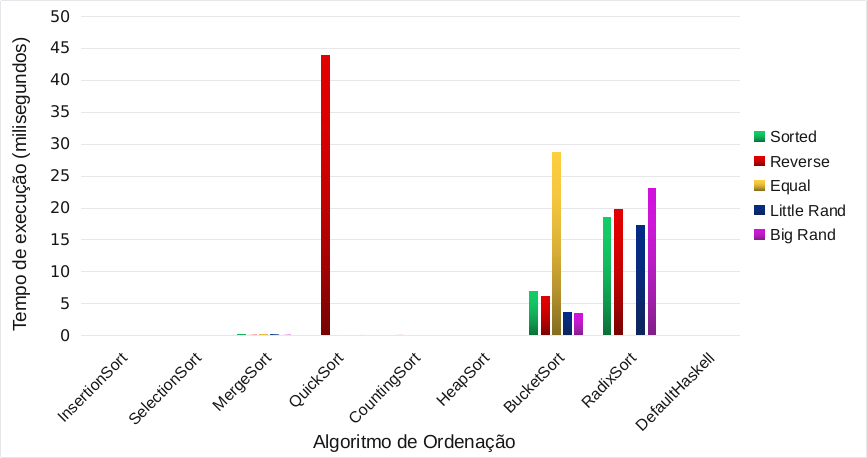
\includegraphics[scale=0.4]{images/result1000-b.png}}
	\caption{Desempenho dos algoritmos para vetores de tamanho 1000}
\end{figure}

\pagebreak

\begin{figure}[h]
	\centering
	\fbox{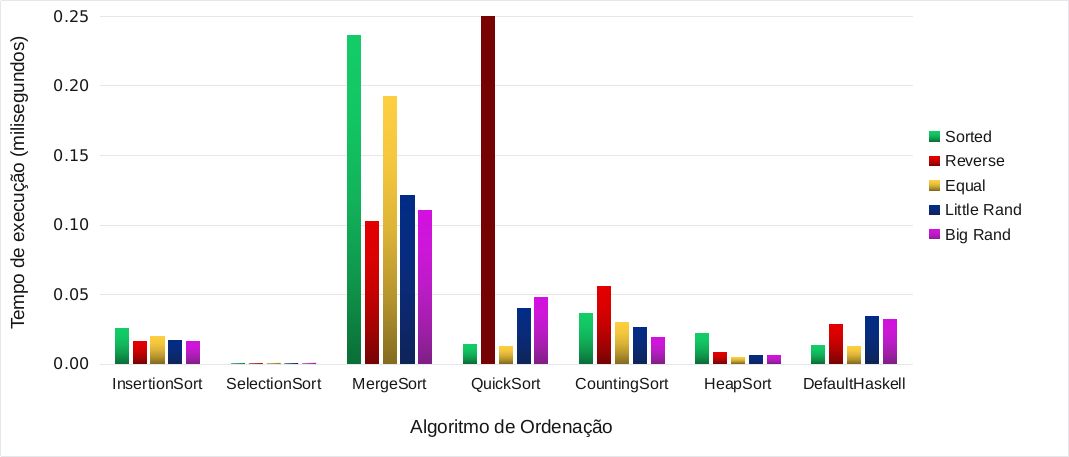
\includegraphics[scale=0.35]{images/result1000-bbkr.png}}
	\caption{Desempenho dos algoritmos mais eficientes para vetores de tamanho 1000}
\end{figure}

O tempo médio do Bubble Sort foi de 1 segundo, cerca de 50 vezes mais lento do que o Radix Sort, que foi o mais lento dentre os outros. Novamente, o Selection Sort se saiu melhor dentre todos os outros algoritmos.

Para os vetores de tamanho 10000, temos:

\begin{figure}[h]
	\centering
	\fbox{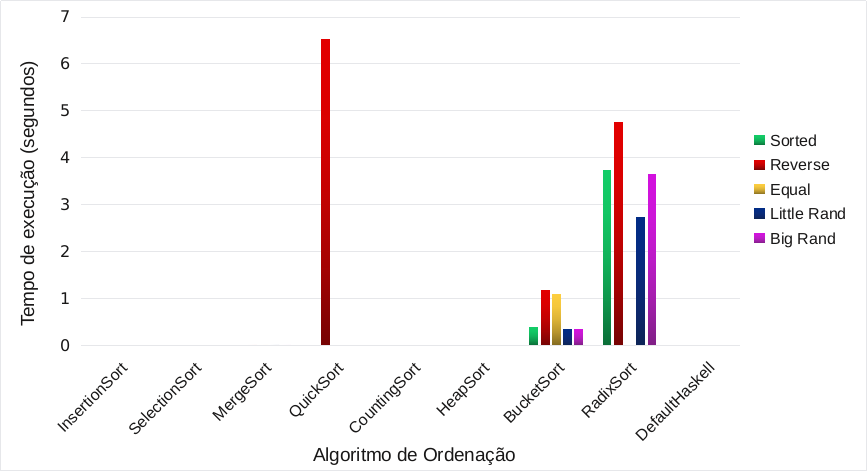
\includegraphics[scale=0.4]{images/result10000-b.png}}
	\caption{Desempenho dos algoritmos para vetores de tamanho 10000}
\end{figure}

\pagebreak

\begin{figure}[h]
	\centering
	\fbox{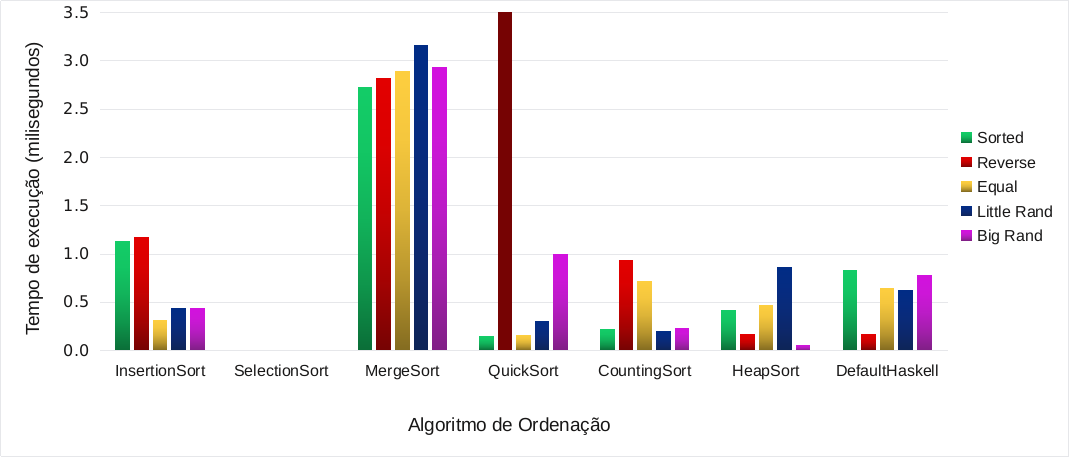
\includegraphics[scale=0.35]{images/result10000-bbkr.png}}
	\caption{Desempenho dos algoritmos mais eficientes para vetores de tamanho 10000}
\end{figure}

O tempo médio do Bubble Sort neste teste foi de aproximadamente 33 minutos, extremamente mais lento do que os demais. Mais uma vez, o Selection Sort demonstrou rápida execução, aparentando seguir um tempo de execução constante em quase todos os testes.

Finalmente, os resultados para os vetores de tamanho 20000 foram os seguintes:

\begin{figure}[h]
	\centering
	\fbox{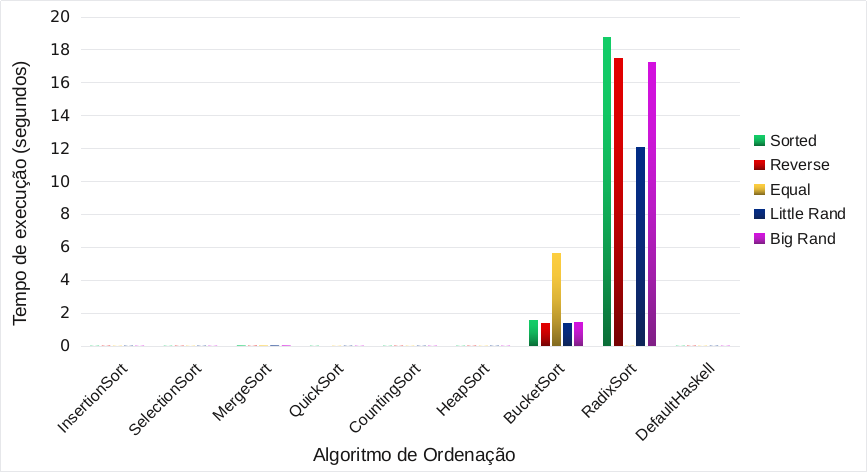
\includegraphics[scale=0.4]{images/result20000-b.png}}
	\caption{Desempenho dos algoritmos para vetores de tamanho 20000}
\end{figure}

\pagebreak

\begin{figure}[h]
	\centering
	\fbox{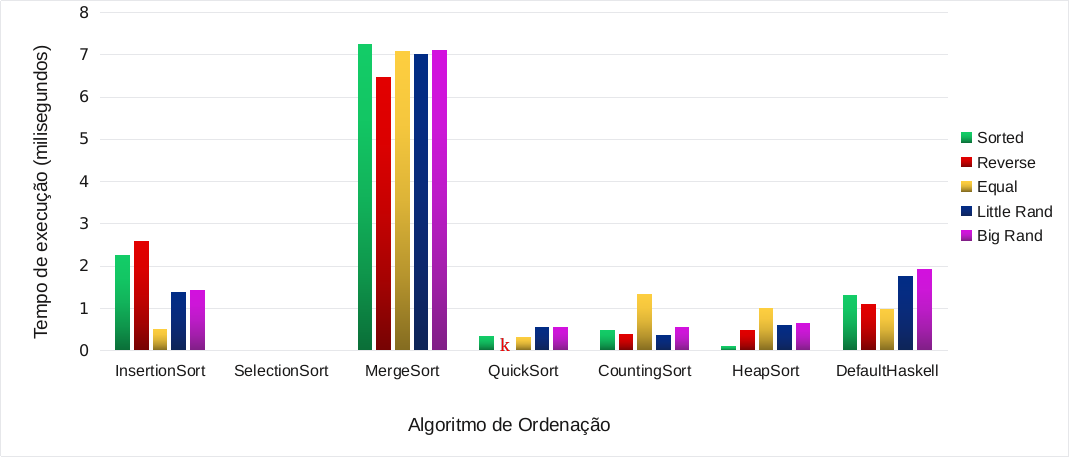
\includegraphics[scale=0.35]{images/result20000-bbkr.png}}
	\caption{Desempenho dos algoritmos mais eficientes para vetores de tamanho 20000}
\end{figure}

Neste caso, o caso pior do Quick Sort (Reverse) foi interrompido pelo próprio stack, que matou o processo. Desta forma, o tempo de execução não pôde ser medido. O tempo médio do Bubble Sort foi de aproximadamente 4 horas e 45 minutos, demonstrando-se um algoritmo muito ruim em termos de velocidade. A revelação ficou por conta do Selection Sort, que manteve o tempo médio de 557 nanosegundos em todos os vetores de teste.

\subsection{Uma variação do Quick Sort}
Visto a ineficiência do Quick Sort perante vetores reversamente ordenados, optou-se por implementar uma variação deste algoritmo, de modo que a primeira tarefa é embaralhar o vetor. Essa é uma solução conhecida e foi aplicada nesse projeto visando comparar sua eficiência com o primeiro Quick Sort adaptado. As funções envolvidas são:

\begin{itemize}
\item \textbf{divide}: Divide o vetor de teste em duas metades, de forma que uma metade contém os elementos de índice par e outra metade contém os elementos de índice ímpar.
\item \textbf{revertePrimeiro}: Recebe as duas metades produzidas pela função anterior e reverte a primeira.
\item \textbf{juntar}: Intercala as duas metades produzidas pelas funções anteriores seguindo uma regra simples aleatória que envolve o tamanho das sublistas.
\item \textbf{shuffle}: Faz a chamada das funções anteriores.
\item \textbf{quickSortShuffle}: Aplica o primeiro Quick Sort implementado neste projeto na lista embaralhada. 
\end{itemize}

Essa variação do algoritmo foi devidamente verificada com o QuickCheck conforme procedimento apresentado na seção 4. Para utilizá-la, necessita-se carregar o arquivo \textbf{src/QuickSortShuffle.hs} com o \textbf{stack} no GHCI. Veja que a sequência de comandos:

\begin{lstlisting}
$ stack ghci src/QuickSortShuffle.hs
$ quickSortShuffle [20,19..1]
\end{lstlisting}

Resulta em:

\begin{figure}[h]
	\centering
	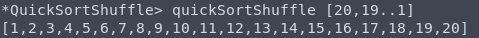
\includegraphics[scale=0.7]{images/qSortShuffle.png}
	\caption{Exemplo de utilização da variação do Quick Sort}
\end{figure}

Através de testes de performance realizados para esta variação com os vetores de tamanho 10000, constatou-se que o tempo médio de execução é de 250 milissegundos para qualquer um dos vetores. É um tempo maior do que o que algoritmo original leva, com exceção do Reverse, que obteve grande redução no tempo. 

\section{Conclusão}
A implementação de algoritmos de ordenação em Haskell pode ser uma tarefa difícil ou fácil, dependendo de muitos fatores. Algoritmos que envolvem estruturas de dados, como o Heap Sort, e algoritmos que trabalham com variáveis mutáveis, como o Counting Sort, o Bucket Sort e o Radix Sort, são especialmente mais difíceis de implementar nesta linguagem funcional utilizando seu conhecimento básico. Em contraposição, algoritmos mais utilizados, como o Quick Sort e outros apresentados em aula tem uma resolução mais elegante, embora nem sempre a eficiência mantenha-se igual em relação às suas implemenetações imperativas. Os algoritmos apresentados neste projeto, da forma que foram implementados, demonstraram eficiência diferente do que se esperava. A partir dos resultados demonstrados na seção 5.2, temos o seguinte ranking de eficiência:

\begin{enumerate}
\item Selection Sort (557 nanosegundos)
\item Quick Sort (0.219 milissegundos)
\item Heap Sort (0.242 milissegundos)
\item Counting Sort (0.280 milissegundos)
\item Default Haskell (0.511 milissegundos)
\item Insertion Sort (0.588 milissegundos)
\item Merge Sort (2.5 milissegundos)
\item Bucket Sort (741.6 milissegundos)
\item Radix Sort (4 segundos)
\item Bubble Sort (1 hora e 21 minutos)
\end{enumerate}

Neste ranking, o tempo é dado pela média dos tempos de execução de todas as listas de teste. Além disso, todos os piores casos do Quick Sort (Reverses) foram desconsiderados. Caso contrário, ele alocaria-se na posição 7, com um tempo médio de 328.5 milissegundos.

Veja que, para os vetores de teste utilizados, o algoritmo padrão de ordenação do Haskell não é o melhor em questões de tempo, embora continue sendo um algoritmo rápido, de resposta quase imediata à nossa percepção. No entanto, como não houve análise de memória utilizada, não há como afirmar se qualquer uma dessas implementações seria de fato melhor do que o algoritmo padrão.

\section{Considerações Finais}
Embora tenhamos feito uma análise de tempo aparentemente justa entre os algoritmos, para alguns deles existem mais fatores que influenciam no seu desempenho. No caso do Bucket Sort, utilizou-se fixamente 10 buckets. Essa quantidade influencia na velocidade do algoritmo, pois se relaciona com o valor máximo presente no vetor. Perceba que para os vetores Equal, o desempenho deste algoritmo foi relativamente ruim, uma vez que todos os algoritmos caíam no mesmo bucket, forçando uma chamada do Insertion Sort puramente para o vetor inteiro.

Além disso, o Radix Sort, que ficou atrás apenas do Bubble Sort, também possui mais fatores que alteram a velocidade da ordenação. Na verdade, é possível dizer que esse algoritmo depende muito mais do número de dígitos do maior número do que de outro fator. Por exemplo, nos vetores de teste Equal, nos quais todos os elementos possuíam apenas um dígito, o Radix Sort foi muito eficiente.

Por fim, embora a metodologia utilizada tenha produzido estes resultados de tempo para os algoritmos implementados, a utilização deles diretamente pelo GHCI parece destoar. Isso porque verifica-se um tempo muito maior para o Selection Sort finalizar uma ordenação do que o apresentado nos testes. No entanto, essa lentidão se verifica no momento de impressão da lista ordenada, de modo que se subentende que a avaliação validada na hora dos testes pelo Main ignorou esta etapa.

\end{document}